% concluding thoughts

\chapter{Impact and Outlook}\label{ch:concl}

\paragraph{Abstract} In the previous chapters we have described the XENON1T detector (Chapter~\ref{ch:xe1t}), two new calibration sources (Chapters~\ref{ch:ng} and~\ref{ch:rn220}), and an off-line analysis to reduce backgrounds from \Rn~(Chapter~\ref{ch:convection}). In this concluding chapter we will discuss the impact these topics have had, as well as prospects for future work.

\section{Neutron Generator}

While the first NR calibration on XENON1T was with an $^{241}$AmBe neutron source~\cite{Aprile:2017iyp}, this was primarily due to technical issues with the neutron generator. The activity of the $^{241}$AmBe source approved for use at LNGS is not very high ($\sim140$~neutrons/second), leading one analysis coordinator to quip that the NR calibration data collected with it was merely background data with NR contamination. Further, $^{241}$AmBe emits neutrons with a broad energy spectrum from $\sim11\1{MeV}$ down to below $100\1{keV}$. The lower-energy neutrons thermalize quickly and are absorbed in the few centimeters of water between the source and the outer cryostat, resulting in a not inconsiderable rate of the $2.2\1{MeV}$ line from capture on $^{1}$H. The neutron generator is not exempt from this, but the lack of low-energy neutrons means fewer neutrons thermalize in the immediate vicinity of the source. Additionally, the adjustable neutron production rate of the generator allows the detector to be calibrated at the maximum rate allowed by the DAQ, minimizing the necessary calibration time. Finally, the quasi-monoenergetic neutron spectrum from the neutron generator allows for accurate \textit{in-situ} measurements of the light and charge yield as reported by LUX~\cite{Akerib:2016mzi}. The generator has been deployed twice on XENON1T at the time of writing, and is now the preferred neutron calibration source. A potential upgrade of the neutron generator would be the addition of a pulsed mode of operation, which would improve the quality of these data by reducing backgrounds.

DD neutron generators will be used on the upcoming $\sim8$~tonne XENONnT and LZ~\cite{Akerib:2018lyp,Mount:2017qzi} experiments, scheduled to enter operation in 2018 and 2019. As these sources are deployed externally to the detector, we do expect a reduction in performance due to the increased detector size. However, the judicious use of a high-energy veto with the DAQ can suppress triggers from events at the edge of the detector in favor of events closer to the center. For the anticipated 50~tonne DARWIN experiment~\cite{Aalbers:2016jon}, the $\sim2.5\1{MeV}$ neutrons from the DD reaction may not be sufficient for a detector of that size, and more study is required on this topic.

\section{$^{220}$Rn source}

The $^{220}$Rn source was designed for use on detectors at the tonne scale or larger where calibration from external sources is impractical or impossible. At the time of writing, it has been deployed on XENON1T a total of 8 times with a combined runtime of over 30 days. These data are primarily used to characterize the low-energy electronic recoil band, utilizing decays of $^{212}$Pb. As leakage from the ER band into the NR band is the dominant source of events in the NR signal region~\cite{Aprile:2015uzo}, the characterization of this signal region is of the utmost importance. $\n{CH_3T}$ was deployed on XENON100~\cite{Aprile:2017xxh}, but the removal of the introduced activity was not as straightforward as expected from the LUX calibration with a similar source~\cite{Akerib:2015wdi}, possibly due to a lack of dedicated methane purification. Though this calibration was performed at the end of the operation of XENON100 and thus did not impact its sensitivity, with even a remote possiblity of a similar outcome for XENON1T the decision was made to not use $\n{CH_3T}$.

Furthermore, this source will be used on the XENONnT and LZ experiments. This source is also expected to be used in the DARWIN experiment, anticipated for 2025, thus demonstrating this source's popularity with future generations of detectors. Based on how the performance of this source scaled from XENON100 to XENON1T, the prospects are promising that scaling up to XENONnT/LZ and even DARWIN will still produce the desired results.

\section{Radon backgrounds in future detectors}

The LZ and XENONnT detectors are expected to be capable of probing a spin-independent WIMP-nucleon scattering cross section of $10^{-48}\1{cm^2}$. As the sensitivity is largely limited by the \Rn-based backgrounds, new methods are required to achieve the necessary radon concentration of $\sim1\1{mBq/tonne}$. Traditionally, the method of radon background reduction was by using materials with lower uranium contaminations~\cite{Aprile:2017ilq,Akerib:2017iwt}. XENON100 demonstrated how online cryogenic distillation could be used to reduce the radon concentration during detector operation~\cite{Aprile:2017kop}, and XENONnT will have a distillation column dedicated for online radon removal.

In Chapter~\ref{ch:convection} we discussed the radon veto, a fundamentally new method of radon background removal. This technique has the distinct advantage of being based on data analysis rather than hardware, and thus can be done even after a detector has ended operation. However, it does cost some exposure which hardware-based methods do not. What remains to be investigated is how a detector's design can be optimized to facilitate the radon veto analysis. For instance, a slower average speed of convection promotes smoother flow patterns in the liquid xenon and suppresses turbulent mixing, which makes following atoms easier. The reduction of convection speed from XENON100 to XENON1T is likely due to improved thermal insulation, and the EXO-200 experiment eliminated convection in their single-phase TPC by immersing the entire cryostat in a cryogen. If convection is entirely eliminated the radon veto reduces to the diffusion-limited case (see Section~\ref{sec:difflimit}), which can effectively eliminate the \Rn~backgrounds at an exposure cost of $<10^{-3}$. The significant reduction of ER backgrounds (and thus leakage into the NR signal region) will be accompanied by a corresponding increase in overall sensitivity.

\section{On the horizon}

Looming some years away is the DARWIN project~\cite{Aalbers:2016jon}, featuring a total of 50~tonnes of xenon. This detector should be capable of probing a WIMP-nucleon cross section of $10^{-49}\1{cm^2}$. While a larger detector could be constructed, as shown in Figure~\ref{fig:darwin_sens}, signals from coherent elastic neutrino-nuclear scattering (CEvNS) represent an unavoidable background of low-energy nuclear recoils, making a search to smaller cross-sections much more difficult. CEvNS is a ready source of low-energy nuclear recoils throughout the entire active volume, and its spectrum mirrors that expected from dark matter interactions, making the identification of a few dark matter events out of several CEvNS events a significant challenge, though an annual modulation search could still be performed.

\begin{figure}[htb]
\centering
    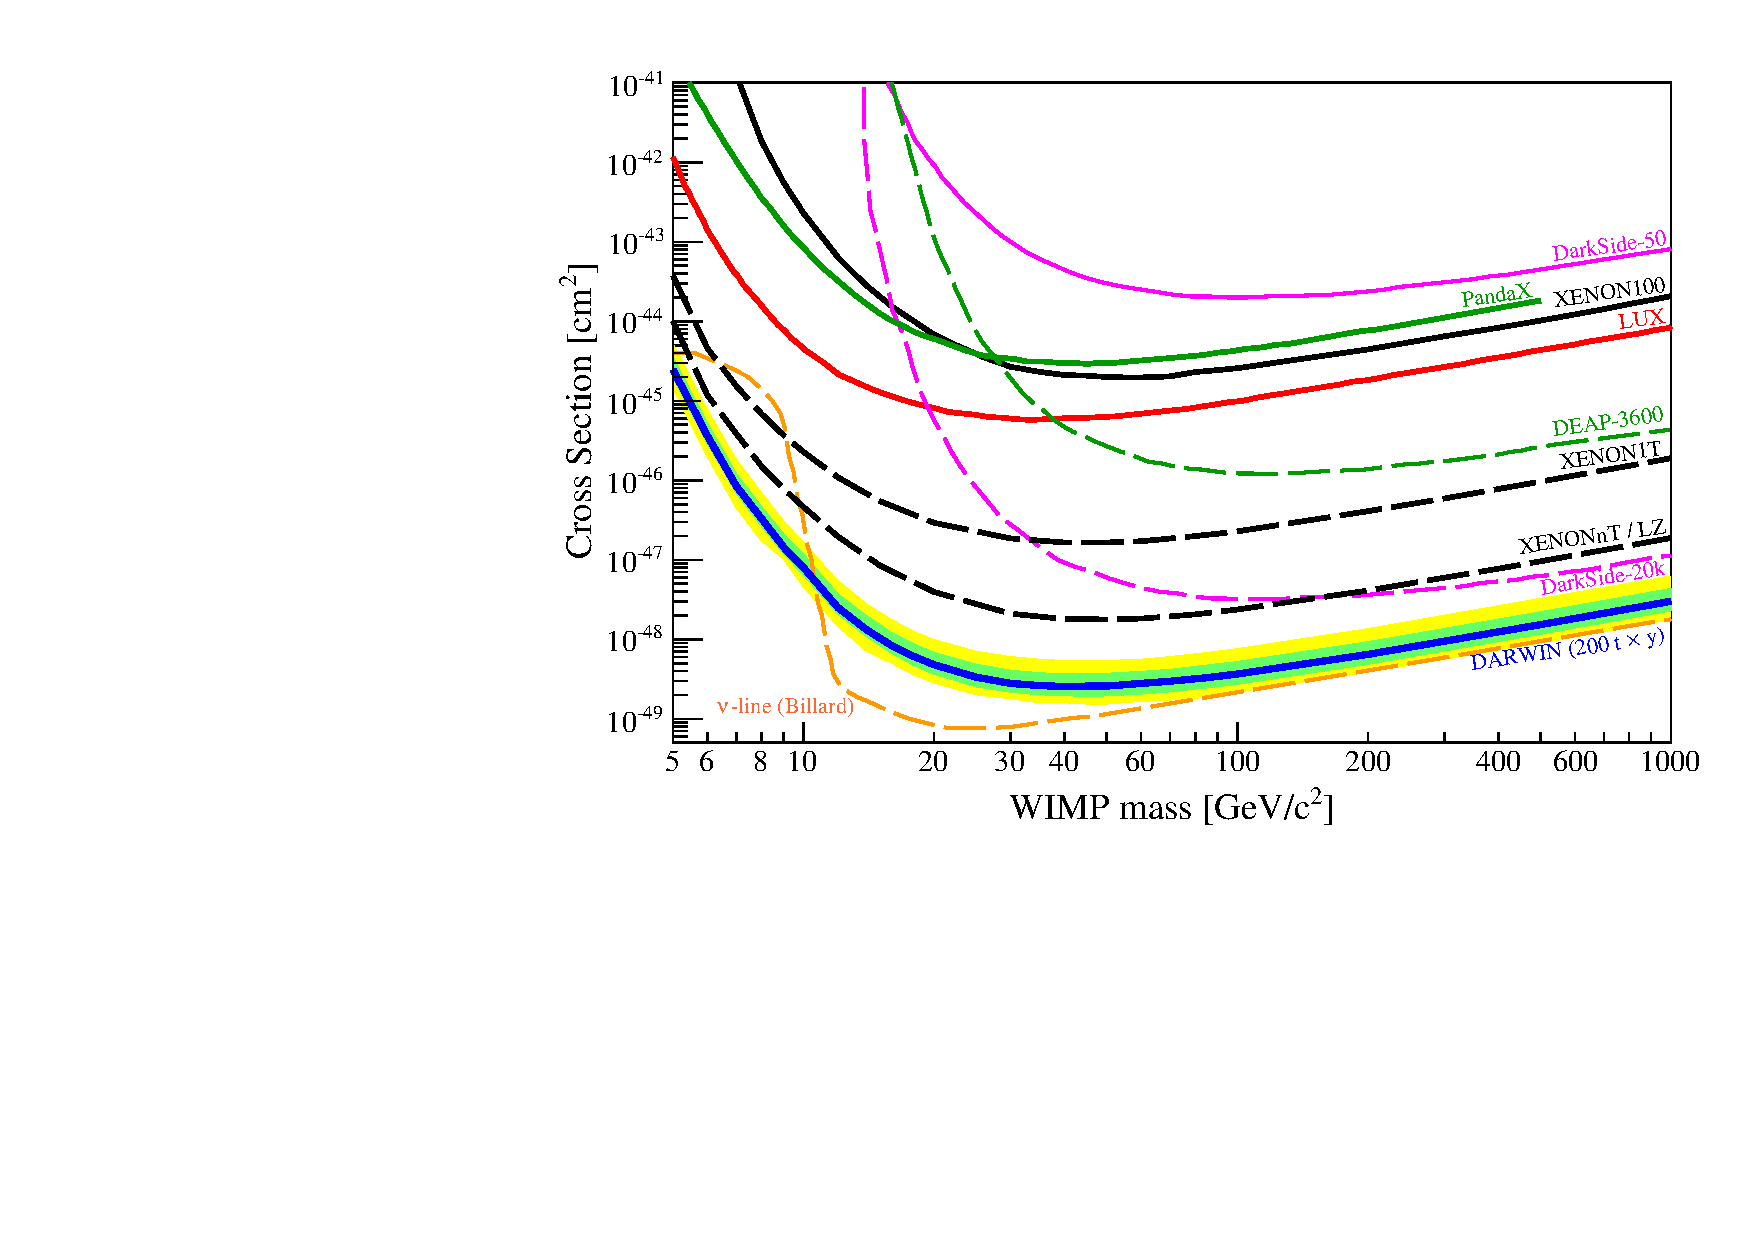
\includegraphics[width=0.8\textwidth]{figures/concl/darwin_sens}
    \caption{Expected sensitivity of the DARWIN experiment to the WIMP-nucleon scattering cross section. While an experiment with a greater sensitivity could be built, it would immediately encounter an unavoidable background from coherent neutrino-nucleus scattering. Figure from~\cite{Aalbers:2016jon}.}\label{fig:darwin_sens}
\end{figure}

A \Rn~concentration of $\sim0.1\1{mBq/tonne}$ is necessary for DAWRIN to reach this sensitivity, two orders of magnitude lower than what was achieved for XENON1T and one order of magnitude lower than what will be required for XENONnT and LZ. Achieving this will require a combination of all of the above techniques, and perhaps new, as yet unknown methods.
